%************************************************
\chapter{The Integration Tier}
\label{ch:integration-tier}
%************************************************

\section{Introduction}

With what we have seen so far, we are able to write server-side components that handle requests from client programs. We know how to structure our code in the presentation tier with the \ac{MVC} design pattern. We also know that we can used \emph{managed components}, for instance \ac{EJB}s to implement the business logic of our application. However, in the examples that we have seen so far, all the data was either generated on the fly or kept in memory data structures. Of course, for real applications we need to be able to interact with persistent data stores, should they be relational or NoSQL databases. The technologies that provide a link between the business services and the databases are located in the \emph{integration tier}, which is the focus of this chapter.

\marginpar{With JDBC, the developer writes SQL queries and sends them to the database. He iterates over tabular results and writes logic to convert records into objects.}

We first introduce the \ac{DAO} design pattern, which is used to decouple the business logic from specific database management systems. We also explain how this pattern can be implemented with a combination of Java EE technologies: \ac{SLSB} to implement the data access services and \ac{JDBC} to submit SQL queries to a database. We also show how the \emph{dependency injection} is used once more, this time to inject a reference to a \emph{data source} into the data access service. 

\marginpar{With an ORM, the developer declares how his object-oriented model is mapped to a set of tables. The ORM generates SQL queries and handles the conversion between records and objects.}

In the second part of the chapter, we introduce the notion of \ac{ORM}, which aims at simplifying the way object-oriented programs interact with relational databases. We illustrate it with the \ac{JPA} standard, which is part of Java EE. We describe how the API offers and alternative to JDBC. We review some of the annotations defined in the specification and discuss some of the tradeoffs to be aware of when deciding to use or not to use an \ac{ORM} solution, and when deciding which features of this solution to use.

\section{Accessing databases from business services}

Let us consider the example of an online shop. One of the use cases is for the customer to land on a \emph{Products} page see a list of products: a small image, a title, a price, ratings, etc. To implement the use case with Java EE, we could go through the following steps:

\begin{itemize}
\item write a servlet that handles the HTTP requests sent to \texttt{/products}
\item write a \texttt{Product} \ac{POJO} class with getter methods
\item write a \texttt{ProductsManager} \ac{SLSB} with a \texttt{List<Product> getProducts()} method
\item write a \ac{JSP} that receives a list of products and renders it in HTML markup
\item wire everything in the servlet, which should obtain a reference to the \ac{SLSB} (usually via dependency injection), make a call to \texttt{getProducts()}, attach the result as model on the request, forwarded to the \ac{JSP}.
\end{itemize}

There is one remaining question however: how should we implement the \texttt{getProducts()} method. This is where we will need to interact with the database. Before looking at solutions, let us consider what are important aspects to consider:

\begin{itemize}
\item \emph{We want to keep our options open and avoid vendor lock-in}. If we write a large application and decide to use a certain type of database, we would like to be able to replace that database with another one in the future. This might mean replacing a \ac{RDBMS} with another \ac{RDBMS} (e.g. replace IBM DB2 with PostgreSQL, or replacing MySQL with Oracle Database). This might also mean replacing a \ac{RDBMS} with a NoSQL database, or vice-versa.
\item \emph{We want to increase the productivity of developers}. Depending on the solution, the developers will have to write more or less code. A solution that automates some of the work and reduces the need for boilerplate code will have a positive impact on productivity. 
\item \emph{We want to have control on non-functional aspects}. If we use a solution that handles some of the work for us, then we must be aware of its impact on performance, scalability and security. We must understand how we can use the right options to control these aspects.
\end{itemize}

\subsection{The Data Access Object pattern}

The \ac{DAO} pattern is extensively used in multi-tiered applications. Whatever the technology stack, you will often encounter codebases with classes following naming conventions based on a variation of \texttt{ProductsDAO}, \texttt{ProductsManager}, \texttt{ProductsRepository} or \texttt{ProductsService}. 

These classes will implement an interface exposing \texttt{CRUD} operations, such as:

\begin{itemize}
\item a method to \emph{create} and store an object in the database
\item a method to \emph{update} an object in the database
\item a method to \emph{delete} an object from the database
\item several methods to \emph{read} one or more objects from the database: by providing a unique id, by providing filtering criteria, etc.
\item possibly additional methods to get the number of objects in the database, perform batch operations, etc.
\end{itemize}

\begin{figure}[]
	\centering
    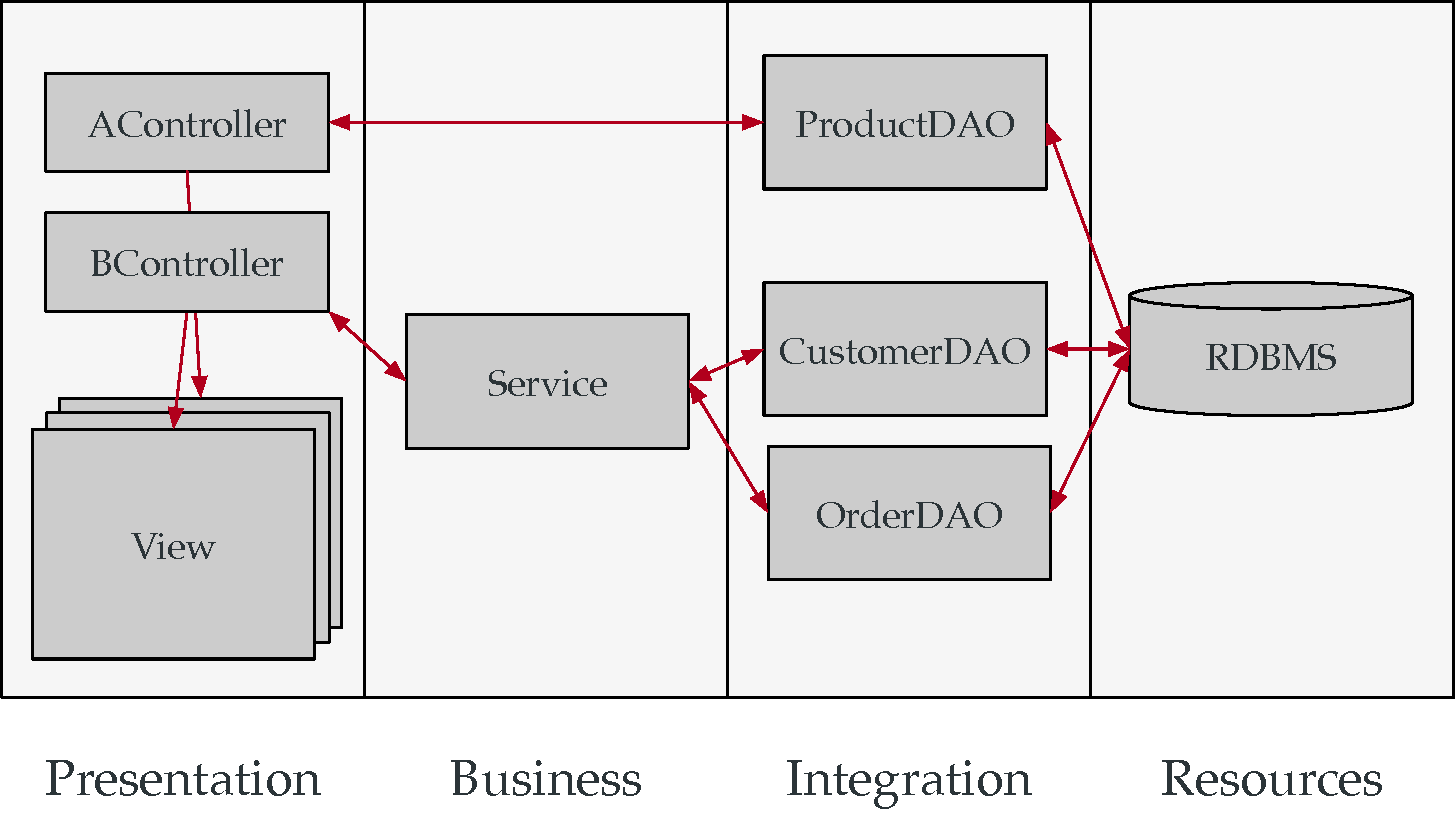
\includegraphics[width=1.0\linewidth]{Figures/dao-in-tiers.pdf}
	\caption{The DAO design pattern}
  \label{fig:daoInTiers}
\end{figure}

Applying the \ac{DAO} pattern allows us to keep the code specific to a particular database technology in a set of well-defined classes. These classes deal only with this \emph{aspect} of the application and are a good example of \emph{separation of concerns}. The way to connect to the database, the way to send queries to the database, the way to process the results are not scattered across the whole codebase. The business services are isolated from the database layer, because they use methods defined in the \ac{DAO} interface. In theory, replacing a database with another database can be as simple as implementing a new \ac{DAO} and injecting a reference to it in the business service. In practice, replacing the database technology may impact non-functional aspects and require some additional work (e.g. to change the frequency at which the \ac{DAO} methods are called).

\subsection{Do we always need a service in the business tier?}

As suggested in Figure \ref{fig:daoInTiers}, some use cases may not require a the implementation of a separate service in the business tier. Indeed, it is possible for a controller in the presentation tier to directly access a \ac{DAO} in the integration tier. But then, how does one decide when to use or to bypass the business tier? There is no clearcut answer to this question, but in general, it is worth implementing a business service when the use case corresponds to a workflow, during which multiple business entities need to be created or modified. In this case, the business service can be seen as a kind of coordinator. What is definitely not worth doing is to create a business service that exposes a \ac{CRUD} interface and simply forwards calls to one \ac{DAO} service. Method names in business services should correspond to business operations: \texttt{registerStudent}, \texttt{sendRewardToGoodStudents} or \texttt{confirmOrder} are such examples.

\subsection{Database resources and connection pools}

When accessing a persistence store, the application needs to establish a connection with the database. One could imagine a scenario where the developer has to load a driver (provided by the database vendor), specify attributes (an IP address and a port, credentials, etc.), open a connection, send a query, receive a result and close the connection. Implemented naively, this scenario would raise two issues:

\begin{itemize}
\item The developer would need to decide where to define connection attributes. Of course, it would be a very bad idea to do that in the code. It would be better to store them in configuration files, but where? Should they be packaged in the \texttt{.war} file? All applications would need to answer this question, which means that a standard solution is valuable.
\item The developer would also be responsible to manage resources very carefuly and deal with non-functional aspects. Under heavy load, he should not open a connection for every request because this would likely starve the database server (which would anyways most likely refuse connection requests at a certain point. Here again, every application developer would need to find an answer to a common problem.
\end{itemize}

Java EE addresses these two issues by making a clear separation between the \emph{development} and the \emph{deployment} phase of an application.

\marginpar{The developers writes code that uses a logical connection named jdbc/myDatabase.}

During the development phase, the developer works with \emph{logical database connections}. In the previous chapter, we have introduced the concept of \emph{dependency injection}. We have seen that when a servlet needs to invoke an \ac{EJB}, it declares a dependency with the \texttt{@EJB} annotation. The application servers injects a reference to managed component at deployment time.

\marginpar{The sysadmin configures the application server: jdbc/myDatabase is mapped to a pool of physical connections to a concrete database server.}

During the deployment phase, the IT ops engineer configures the application server, configures \emph{physical database connections} and defines a mapping between logical and physical connections. This is when he specifies the connection parameters (IP address, port number, credentials, etc.). This 
is also when he configures how connections are to be pooled (so that they can be shared and reused by different clients).

\begin{figure}[]
	\centering
    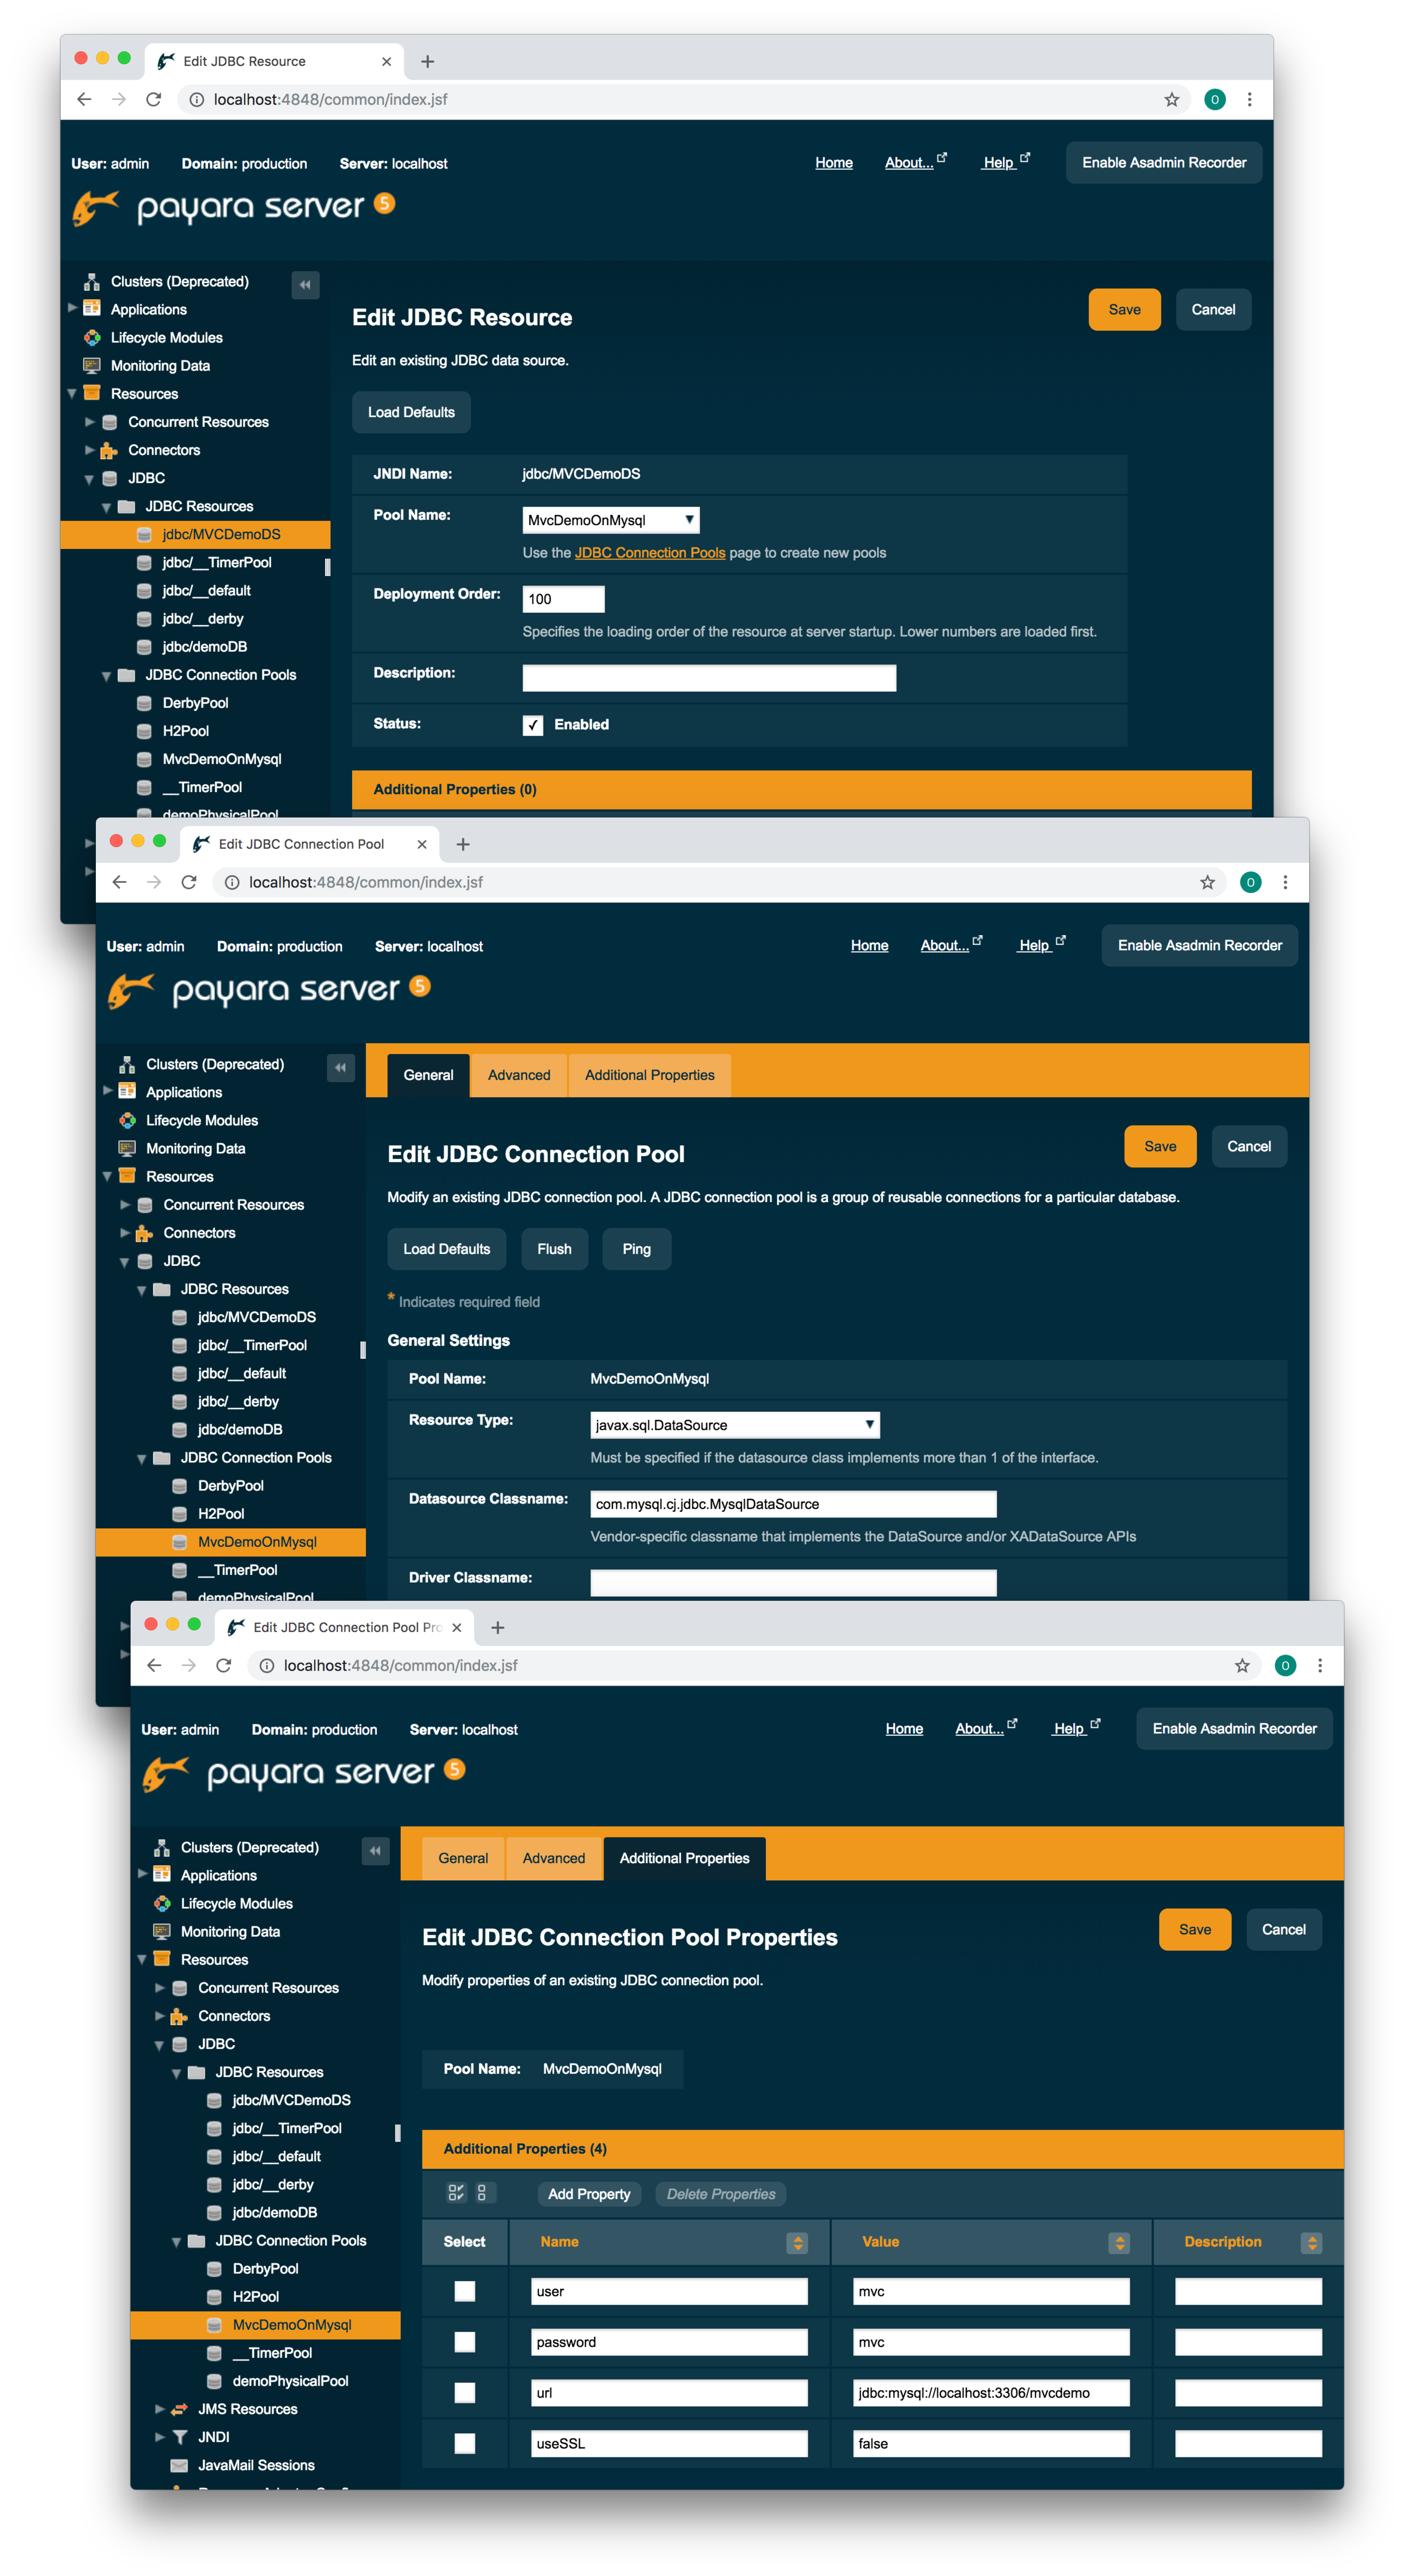
\includegraphics[width=1.0\linewidth]{Figures/screenshot-jdbc.pdf}
	\caption{The JDBC resource maps a logical name to a connection pool}
  \label{fig:jdbcResource}
\end{figure}

\subsection{The Java DataBase Connectivity API}

\ac{JDBC} is almost as old as Java: the first version of this API was part of the Java Development Kit 1.1 in 1997. The current version is JDBC 4.3 and is part of Java SE 9. \ac{JDBC} was proposed to enable Java applications to interact with relational database management systems in a standard way. In other words, the goal was to allow developers to write data access logic once and to use it with databases from different vendors. In other words, the application should be able to store its data in a DB2 database, in an Oracle database or in MySQL database without any code change. To achieve this goal, \ac{JDBC} defines both an \ac{API} and a \ac{SPI}. The \ac{API} is the interface used by application developers. It defines operations to open connections, to send queries, to receive results, etc. The \ac{SPI} is the interface used by database vendors. It defines operations that have to be implemented in \ac{JDBC} \emph{drivers}.

\marginpar{Java EE applications do not use the \texttt{DriverManager} class. Instead, they use \texttt{DataSource} objects, which are injected in the services that contain data access logic.}

Figure \ref{fig:jdbcDriver} shows how the \ac{JDBC} driver provides an abstraction layer between the application code and a specific database management system. The application code only uses the \ac{API}. Since all drivers have to implement it, the same application can interact with different applications, just by switching the driver. This raises an interesting question: how are drivers loaded and how does the application specify that it wants to use one particular driver? The code in the diagram describes what happens (note that the situation is a bit different since \ac{JDBC} 4, but the general idea remains the same).

\begin{figure}[]
	\centering
    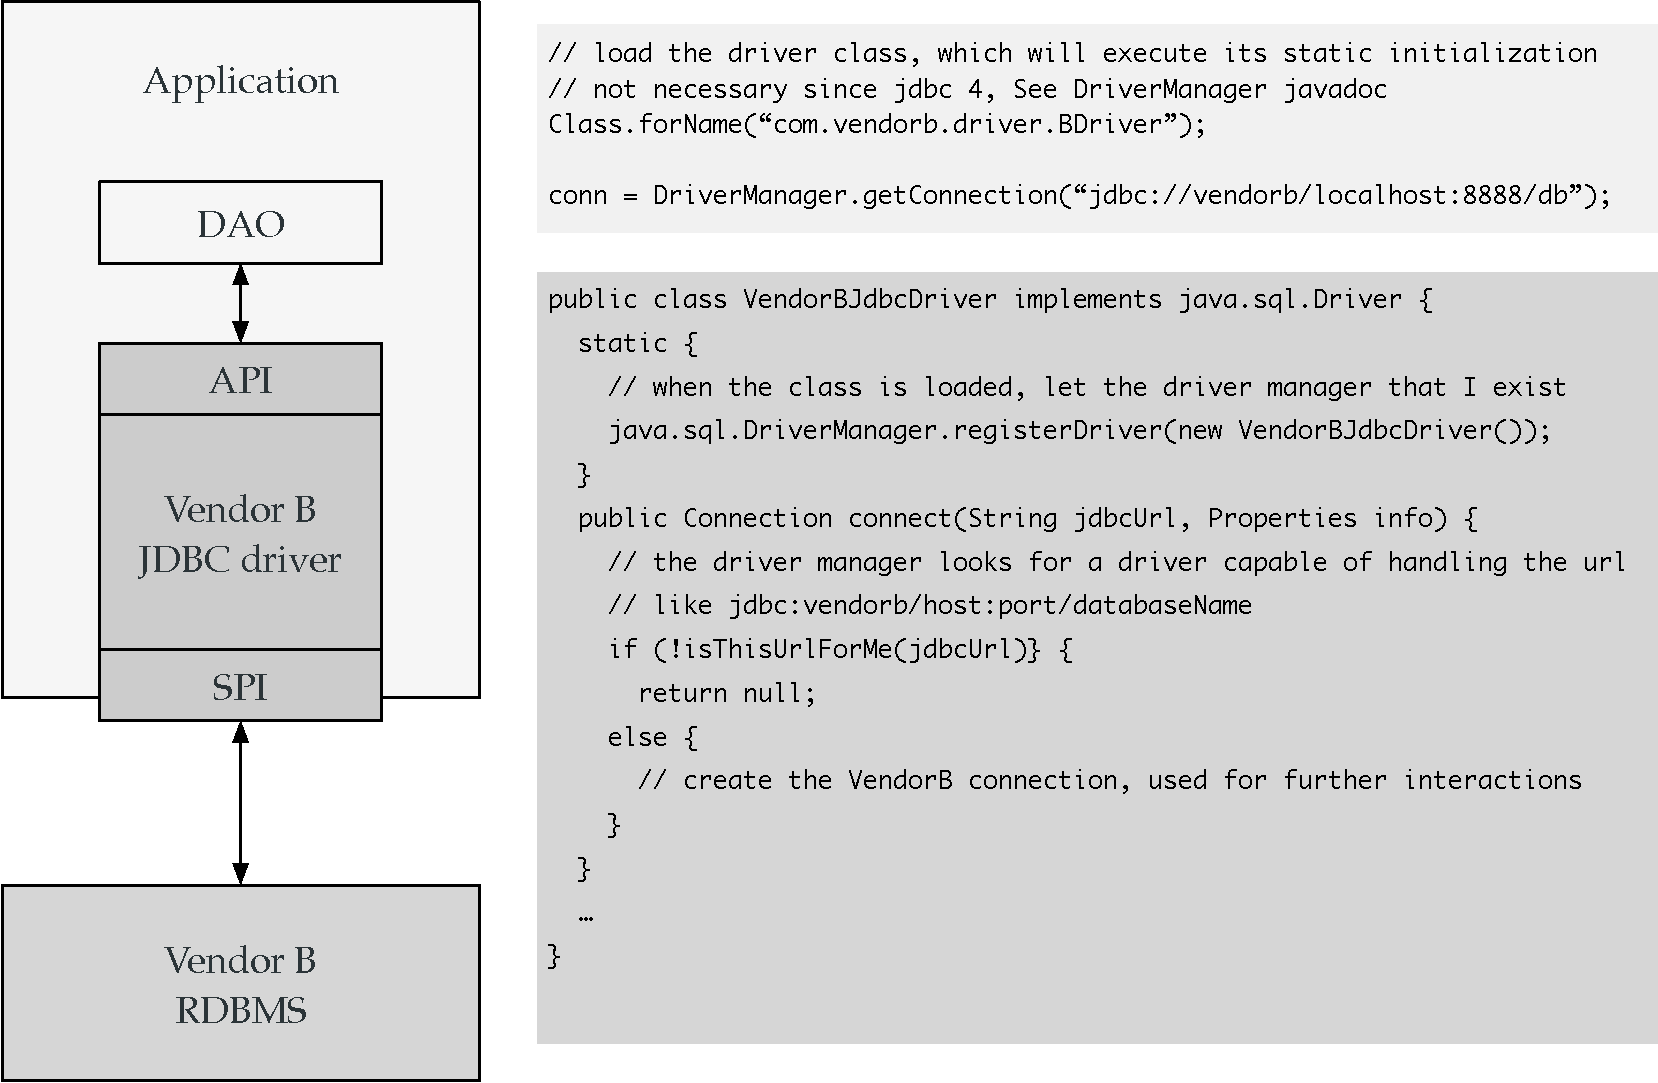
\includegraphics[width=1.0\linewidth]{Figures/jdbc-driver.pdf}
	\caption{JDBC provides an abstraction layer between the application and the database}
  \label{fig:jdbcDriver}
\end{figure}


\subsection{Putting things together: implement a DAO with EJB and JDBC}

\lstset{
	caption={Implement a DAO with a Stateless Session Bean},
	language=java,
	label={lst:daoWithEJB}
}
\vspace{10pt}
\begin{minipage}{\linewidth}
\begin{lstlisting}[frame=single]
@Stateless
public class SensorJdbcDAO implements SensorDAOLocal {

  @Resource(lookup = "jdbc/AMTDatabase")
  private DataSource dataSource;

 public List<Sensor> findAll() {
    List<Sensor> result = new LinkedList<>();
    try {
      Connection con = dataSource.getConnection();

      PreparedStatement ps = con.prepareStatement("SELECT * FROM Sensors");
      ResultSet rs = ps.executeQuery();

      while (rs.next()) {
        Sensor sensor = new Sensor();
        sensor.setId(rs.getLong("ID"));
        sensor.setDescription(rs.getString("DESCRIPTION"));
        sensor.setType(rs.getString("TYPE"));
        result.add(sensor);
      }

    } catch (SQLException ex) {
      Logger.getLogger(SensorJdbcDAO.class.getName()).log(Level.SEVERE, null, ex);
    } finally {
      if (ps != null) { ps.close(); }
      if (con != null) { con.close() };
    }
    return result;
  }
}
\end{lstlisting}
\end{minipage}

\begin{itemize}
\item Line 1: the DAO is a \ac{SLSB}. This is particularly important from a transaction demarcation point of view. The container starts a transaction whenever a business method is called and commits it if the method returns a result. If the method throws an exception, then the container rollbacks the transaction.
\item Lines 4-5: we inject a dependency on the data source. The container will assign a value to the dataSource variable. This will work only if the administrator has configured a \ac{JDBC} connection in the application server.
\item Line 7: we have not implemented a complete \ac{CRUD} service, but only implemented a finder method.
\item Line 10: we ask for a connection from the pool. Under heavy traffic, we might have to wait for one to become available (this will avoid that we overload the database server).
\item Lines 12-13: we prepare a SQL query, send it to the server, receive a list of records.
\item Lines 15-21: we iterate over the records and at each iteration, we create a \ac{POJO} model object. We transfer data from the \ac{JDBC} record to the model.
\item Lines 23-24: we close the resources. Note that in reality, this will not close the connection but rather return it to the pool, so that it can be reused for another request.
\end{itemize}

\section{Object Relational Mapping}

TODO: content will be published later.


\section{Questions}

To answer these questions, you will need to have read the chapter but also to have done some research. Make sure that you are able to answer every question. Discuss your responses with your peers.


